\chapter{Introduction}
\section{Section 1}
Language is infinite \citep{yang2006infinite} and its sound systems can be analyzed with features \citep{chomsky1968sound}. \lipsum[1]

\begin{figure}[ht]
    \centering
    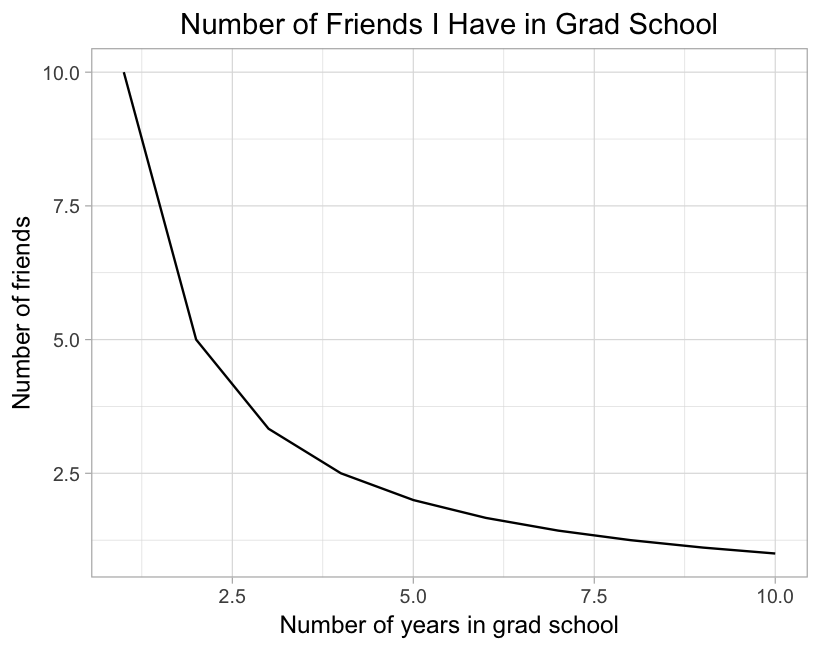
\includegraphics[scale=0.3]{friends}
    \caption{This is an example figure.}
    \label{fig:friends}
\end{figure}

\subsection{A Subsection}
\lipsum[2]
\subsubsection{A Subsubsection}
Table \ref{tbl:sepalwidth} summarizes the statistics. \lipsum[22] 

% latex table generated in R 3.5.0 by xtable 1.8-2 package
% Sat Aug 25 07:47:40 2018
\begin{table}[ht]
\centering
\begin{tabular}{rlrrrrr}
  \hline
 & Species & N & Sepal.Width & sd & se & ci \\ 
  \hline
1 & setosa & 50.00 & 3.43 & 0.38 & 0.05 & 0.11 \\ 
  2 & versicolor & 50.00 & 2.77 & 0.31 & 0.04 & 0.09 \\ 
  3 & virginica & 50.00 & 2.97 & 0.32 & 0.05 & 0.09 \\ 
   \hline
\end{tabular}
\caption{This is a table.}
\label{tbl:sepalwidth}
\end{table}

\subsection{A Second Subsection}
\lipsum[3]
\section{Section 2}
\lipsum[4]
\subsection{Another Subsection}
\lipsum[5-7]


